\documentclass[11pt,a4paper]{article}
\usepackage{fontspec}
\usepackage[english]{babel}
\usepackage[margin=2.1cm]{geometry}
\usepackage{booktabs,array,tabularx}
\usepackage{xcolor}
\usepackage{graphicx}
\usepackage{pgfplots}
\pgfplotsset{compat=1.17}
\PassOptionsToPackage{hyphens}{url}
\usepackage[hidelinks]{hyperref}
\usepackage{enumitem}
\setlist{nosep,leftmargin=1.4em}
\emergencystretch=3em

\definecolor{impl}{HTML}{3B6EA8}
\definecolor{rev}{HTML}{8FB3DA}

\title{Sweatshop on P-Chess: the UI redo's game screens\\\large Home, name dialog and searching (UI-022), game screen board and side panel (UI-023) and game-over card (UI-024); GPT-6.1 Terra lineup, lane \texttt{ui-game}}
\author{Foreman, session \texttt{sweatshop/ui-game/2026-10-31-1734}}
\date{31 October 2026}

\begin{document}
\maketitle

\section*{Summary}

First run of the \texttt{ui-game} lane, in its clone at \path{.artifacts-build/lanes/ui-game},
side by side with the \texttt{ui-review} and \texttt{ui-screens} lanes. UI-021 (the shared theme)
was already on \texttt{main}. Launch at 17:34, last merge at 19:19, session PR
\href{https://github.com/Laginho/P-Chess/pull/36}{\#36}.

\begin{itemize}
  \item \textbf{Produced:} the three lane tickets merged on the session with
        \texttt{Verdict: Approve}: UI-022, UI-023 (\texttt{Review: human}, still waiting for
        Bruno) and UI-024. Gate 416 executed, 0 failed, 7 skipped (6 need Lc0, 1 needs a display);
        413 passed before the run.
  \item \textbf{Cost:} \textbf{\$9.03} at API list price over 12 stages, all priced:
        \texttt{gpt-6.1-terra xhigh} implementing \$4.54 (6), \texttt{gpt-6.1-sol xhigh} reviewing
        \$4.49 (6). Codex quota: 8 points of the weekly window (Terra xhigh 4, Sol xhigh 4;
        $\pm$1 per stage, the total is exact), no reset; 2 Codex rollouts outside the stages,
        0 points. Two sibling lanes ran on the same account at the same time.
  \item \textbf{What went wrong:} every ticket was reopened once, all for real defects, and two of
        the four findings were the same one: a long player name cut off at 800$\times$600
        (UI-022, then UI-024, whose implementer had noted the risk in its own handoff and left
        it). UI-022's review also showed that UI-021's font weights never render; the fix is
        CLEAN-012, filed outside this lane, and it holds PR \#36 off \texttt{main}.
  \item \textbf{Provisional verdict:} Terra xhigh again reached review on every first attempt
        (3 of 3, 11--27~min), no early stop. Its fixes took 5--6~min. Its pair with Sol xhigh is
        now 35\% reopened over 17 reviews.
\end{itemize}

\section*{What was done}

\textbf{UI-022}: Home, the first-launch name dialog and the searching screen now follow the
v0.1.0 design: the board on the left, the title, the Maia level selector, a 2$\times$2 grid of
quick-play buttons with icons, and History, Profile, Settings and Quit with icons below; the
searching card has a spinner, ``Starting your game'', the live status and chips for time control
and level. Main files \path{ui/home.tscn}, \path{ui/name_dialog.tscn}, \path{ui/searching.tscn}.
Reopened once: a long player name ran past the searching card and the window at 800$\times$600;
the player label in \path{ui/searching.gd}/\path{ui/searching.tscn} had no width bound. It now
ends in an ellipsis and the full name stays saved.

\textbf{UI-023}: the game screen: Lichess brown board with the design's last-move colours,
coordinates inside the squares and the resize grip's icon; a side panel card with both players'
rows (score box, avatar, name, clock; the running clock is the light one), the move list as a
numbered table, Offer draw and Resign with icons, a red ``Click again to resign'' with a draining
bar, and the ``Maia declined''/``Draw agreed'' notice. The in-game Settings button, the material
counters and the side Review button are gone, as Bruno decided, with \path{tests/test_material.gd};
\path{docs/spec.md} §8.4, §8.7, §9.2 and §9.3 say so. Main files \path{ui/main.tscn},
\path{ui/main.gd}, \path{ui/move_list.gd}, \path{ui/board_view.gd}. Reopened once for two
regressions of its own change: each new move threw the move list back to the end even when you
had scrolled up to read (\path{ui/move_list.gd} rebuilt the table), and after a rematch in F11
focus mode the previous game's draw notice came back and stayed (\path{ui/main.gd} did not clear
the saved notice).

	extbf{UI-024}: the game-over card: a head tinted by the result with a trophy, flag or one-half icon, both
players with avatars and the winner ringed in gold, the match score, a green ``Review'' button
with ``New game'' and ``Rematch'' below, Copy PGN at the top left (the review's action) and a
close button. Main files \path{ui/game_over.tscn}, \path{ui/game_over.gd}. Reopened once: long
player names were cut at both ends with no ellipsis (\texttt{clip\_text} in
\path{ui/game_over.tscn}).

\section*{Timeline}

{\small
\begin{tabularx}{\linewidth}{@{}lX@{}}
\toprule
17:25 & Lane clone made, assets imported, baseline gate 413 passed. \\
17:34 & Launch, default lineup (Terra), pid 29104; proxy pinged, Codex sessions reach it directly. \\
18:01--18:08 & UI-022 to review (27~min), reopened (long name on Searching); CLEAN-012 filed. \\
18:13--18:19 & UI-022 fixed in 5~min, merged (proxy: merge into the session, CLEAN-012 holds \texttt{main}). \\
18:19--18:25 & UI-023 stage 2 asks the proxy twice (scope of \path{ui/game_over.gd} and \path{scripts/screens.gd}). \\
18:40--18:45 & UI-023 to review (21~min), reopened (move-list scroll, stale notice). \\
18:51--18:54 & UI-023 fixed in 6~min, merged. \\
19:05--19:12 & UI-024 to review (11~min), reopened (long names on the card). \\
19:16--19:19 & UI-024 fixed in 5~min, merged. Nothing left; PR \#36 (3 tickets). \\
\bottomrule
\end{tabularx}
}

\section*{Per stage}

{\small
\begin{tabularx}{\linewidth}{@{}llllrrrrrX@{}}
\toprule
When & Ticket & Stage & Model & Min & In & Cache & Out & Cost & Outcome \\
\midrule
18:01 & UI-022 & impl & terra xhigh & 27 & 28.4M & 99\% & 50k & 1.81 & to-review \\
18:08 & UI-022 & review & sol xhigh & 6 & 4.7M & 95\% & 23k & 1.10 & reopened \\
18:13 & UI-022 & impl & terra xhigh & 5 & 3.7M & 98\% & 7k & 0.30 & to-review \\
18:19 & UI-022 & review & sol xhigh & 5 & 2.1M & 94\% & 14k & 0.58 & merged \\
18:40 & UI-023 & impl & terra xhigh & 21 & 19.2M & 99\% & 43k & 1.30 & to-review \\
18:45 & UI-023 & review & sol xhigh & 5 & 4.0M & 95\% & 20k & 0.98 & reopened \\
18:51 & UI-023 & impl & terra xhigh & 6 & 4.4M & 98\% & 9k & 0.33 & to-review \\
18:54 & UI-023 & review & sol xhigh & 3 & 1.5M & 93\% & 10k & 0.46 & merged \\
19:05 & UI-024 & impl & terra xhigh & 11 & 8.5M & 99\% & 24k & 0.62 & to-review \\
19:12 & UI-024 & review & sol xhigh & 6 & 3.3M & 95\% & 20k & 0.84 & reopened \\
19:16 & UI-024 & impl & terra xhigh & 5 & 2.3M & 98\% & 5k & 0.19 & to-review \\
19:19 & UI-024 & review & sol xhigh & 3 & 1.8M & 93\% & 12k & 0.54 & merged \\
\midrule
 & & & & 103 & 83.9M & & 237k & 9.03 & \\
\bottomrule
\end{tabularx}
}

\begin{center}
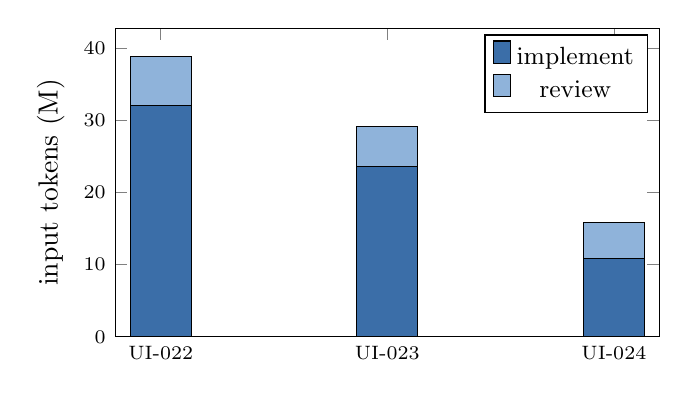
\begin{tikzpicture}
\begin{axis}[ybar stacked, bar width=22pt, width=0.7\linewidth, height=5.5cm,
  symbolic x coords={UI-022,UI-023,UI-024},
  xtick=data, ylabel={input tokens (M)}, ymin=0, legend style={at={(0.98,0.98)},anchor=north east,font=\small},
  tick label style={font=\scriptsize}]
\addplot[fill=impl] coordinates {(UI-022,32.1) (UI-023,23.6) (UI-024,10.8)};
\addplot[fill=rev] coordinates {(UI-022,6.8) (UI-023,5.5) (UI-024,5.1)};
\legend{implement, review}
\end{axis}
\end{tikzpicture}
\end{center}

Wasted: no failed or asked stage. The three reopens cost a fix and a second review each
(\$0.82 + \$0.79 + \$0.73 = \$2.34, 26\% of the run); UI-024's could have been avoided, since its
implementer named the defect and handed it on. Input is 79\% implementation, mostly cached.

\section*{Comparison with previous runs}

From \texttt{run-log.md}. The \texttt{v010} lane's run~3 (9 tickets) cost \$2.30 per merged
ticket; this run \$3.01, with every ticket reopened (6 of 9 there). Terra xhigh's first stage 2
took 27, 21 and 11~min here against 11--12~min there; these screens touch more scenes and
capture screenshots at two sizes. Fixes after a reopen took 5--6~min, as before (4--9). Reviews
cost \$0.46--1.10 (\$0.46--1.05 there). The \texttt{ui-base} lane's UI-021 cost \$2.48 in two
stages.

\section*{Observations per model}

\begin{itemize}
  \item \textbf{gpt-6.1-terra xhigh, stage 2} (6 stages, 3 tickets): every stage reached review,
        every fix test-first with the red run recorded. Two of its four findings were regressions
        next to its own change (UI-023), two were the same 800$\times$600 long-name check, which it
        did not run on UI-024 although it wrote ``Long player names can be clipped'' in that
        handoff and UI-022 had just been reopened for it. It asked the proxy twice on UI-023 for
        files outside the Primary list, both needed.
  \item \textbf{gpt-6.1-sol xhigh, review} (6 stages, 3--6~min): every reopen was reproduced with
        a probe and numbers (label rects, scroll offsets, notice state). It found and proved the
        UI-021 font-weight miss (TextServer reports no applied axis) and filed CLEAN-012 instead of
        fixing outside the ticket. It reused gate receipts and did not rerun the display-only
        pixel test; the foreman ran it (Acceptance).
\end{itemize}

\section*{Driver and runtime issues}

\begin{enumerate}
  \item None in the driver: no crash, no timeout, no API error, no parked handoff. Shutdown
        1.0--1.8~s per stage.
  \item The new clone needed \texttt{godot --headless --import} and \texttt{*.uid}/\texttt{*.import}
        in \path{.git/info/exclude} before its tree was clean; the import rewrote
        \path{fonts/NotoSans-Variable.ttf.import} with LF endings (restored by checkout).
  \item Lc0 is not in the clone: the six engine tests skip and no stage played a real game.
  \item Every screenshot was written to \path{%TEMP%}. The foreman copied the before, after and
        reference PNGs to \path{.artifacts-build/ui-game-screens/} (ignored) so they outlive a
        temp cleanup.
\end{enumerate}

\section*{Recommendations}

\begin{enumerate}
  \item Run CLEAN-012 (shared font weights, \path{ui/theme/p_chess.tres}) before PR \#36 merges:
        every ticket here records it as an integration condition. It sits in
        \path{.scratch/ui-base/issues/} with prefix \texttt{74}, the same as UI-022's file;
        renumber it when it runs.
  \item Add ``a long player name at 800$\times$600'' to the shared acceptance in
        \path{.scratch/ui-redo/spec.md}: it reopened two of three tickets here, and History,
        Review and Profile also show the name.
  \item Ticket the display-only failure of
        \texttt{test\_editor\_right\_click\_\allowbreak refreshes\_tree\_and\_board} in
        \texttt{test\_repertoire.gd}: with a
        real display it fails on \texttt{main} too (2 assertions), so it is not this lane's, but the
        headless gate never sees it.
  \item Keep screenshot evidence in an ignored folder of the repo instead of \path{%TEMP%}
        (\path{scripts/screens.gd} usage in \path{docs/design/v0.1.0/README.md}).
\end{enumerate}

\section*{Human debt and proxy decisions}

No \texttt{Débito humano:} lines in this run's tickets. Three proxy decisions, all by
\texttt{opus-5.5 xhigh}, asked by the stages themselves (Codex reached the proxy directly):

\begin{itemize}
  \item UI-022: \texttt{Proxy decided (opus-5.5 xhigh)}: ``Approve UI-022 and close it the normal
        way: merge into the session branch, add the ledger line, set \texttt{Stage: done}, and keep
        the CLEAN-012 disclosure at \texttt{pending | integration} — integration means the session
        PR landing on \texttt{main}, and merging into the session branch is not that.''
  \item UI-023: \texttt{Proxy decided (opus-5.5 xhigh)}: ``Yes. Add \path{ui/game_over.gd} and
        \path{scripts/screens.gd} to Primary files, scoped to removing the side Review button and
        updating the one call site. No restyling. Criterion 4 can't pass without them.''
  \item UI-023: \texttt{Proxy decided (opus-5.5 xhigh)}: ``Yes, widen the
        \path{scripts/screens.gd} scope for the four UI-023 boards — the fixture should show the
        game screen the way \texttt{\_start} leaves it, or shared acceptance 1 and 4 compare against
        a state the app never shows.''
\end{itemize}

\section*{Acceptance}

Probes on the session head \texttt{be29801}: the headless gate (416 executed, 0 failed, 7
skipped); the full suite with a display, where
\texttt{test\_last\_move\_uses\_the\_two\_design\_colours} passes (\#cdd26a light, \#aaa23a dark)
and the one failure is the pre-existing repertoire test above (it fails on \texttt{main}
\texttt{acb4662} too). Reviews checked 1280$\times$800 and 800$\times$600 captures against the
reference PNGs for all ten boards, with differences listed in each ticket. Not examined: real play
with Lc0, physical input, audio, and Bruno's visual comparison; final visual acceptance waits on
CLEAN-012.

\section*{Reopen attribution}

Labelled by the foreman (opus-5.5); the reviewer was \texttt{gpt-6.1-sol xhigh}, so no
self-judging. Rows appended to \path{.scratch/reopen-attribution.md}.

{\small\noindent
\begin{tabularx}{\linewidth}{@{}>{\raggedright\arraybackslash}p{1.7cm}X>{\raggedright\arraybackslash}p{2.7cm}X@{}}
\toprule
Ticket (round) & Finding & Label & Why \\
\midrule
UI-022 (1) & Long name overflows the Searching card at 800$\times$600 & S2-explícito/\allowbreak código ? & criterion 4 carries ``nothing clipped at 800$\times$600''; borderline, long names not named \\
UI-023 (1) & New move throws the move list back to the end & S2-implícito & regression of its own table rewrite \\
UI-023 (1) & Old draw notice returns after a rematch in focus mode & S2-implícito & cleanup path of state it kept for focus mode \\
UI-024 (1) & Long names clipped on the card, no ellipsis & S2-explícito/\allowbreak código & criterion 5; disclosed by stage 2 and left \\
\bottomrule
\end{tabularx}
}

Totals, reopens: S2-explícito/código 2 (one borderline), S2-implícito 2, S1 0, S3-ruído 0;
fixed in review: none. No review-induced churn, no drip-feed. One post-approval finding, recorded
as \texttt{session-review}, \texttt{unclassified}, review miss \texttt{yes}: UI-021's font weights
(criterion 2) never applied; its approval checked the resource, not the rendered axes. Found by
UI-022's review after PR \#33 merged; follow-up CLEAN-012.

\section*{Scoreboard}

\texttt{scoreboard.ps1} over the ClassyCall, EasyMath, PhysiSyst, SIGAA-ME and SynchroNice main
checkouts plus this lane's clone in place of P-Chess's main checkout (same merged run log; it
holds this run's attribution rows before they reach \texttt{main}). Moved since the \texttt{v010}
run~3 report: implementer \texttt{gpt-6.1-terra xhigh} 11 $\to$ 18 stage runs, 0 failed, 1 asked
(earlier); pair \texttt{gpt-6.1-terra xhigh} $\rightarrow$ \texttt{gpt-6.1-sol xhigh} 10 $\to$ 17
reviews, 30\% $\to$ 35\% (S2 rate 35\%, fixed in review 2, UI-021's included); the same reviewer
over \texttt{gpt-6.1-terra high} stays at 30\% (20 reviews) and over \texttt{gpt-6.1-sol high} at
23\% (22). Both Terra pairs now sit 7--12 points above Sol high under the same reviewer, each over
17 or more reviews. Interventions: automatic-recovery 101 $\to$ 110, proxy-decision
(opus-5.5 xhigh) 6 $\to$ 11 (other lanes included).

{\tiny
\begin{verbatim}
| Implementer | Stage runs | To review | Failed | Asked | Median min to review | Cost |
|---|---|---|---|---|---|---|
| gpt-6.1-sol high | 68 | 63 | 0 | 5 | 9m | $47.66 (68/68 priced) |
| opus-5.5 medium | 3 | 2 | 1 | 0 | 6m | $4.79 (3/3 priced) |
| opus-5.5 | 7 | 4 | 0 | 3 | 14m | $15.12 (7/7 priced) |
| gpt-6-luna max | 89 | 61 | 10 | 18 | 17m | $4.91 (85/89 priced) |
| sonnet-5.5 high | 2 | 2 | 0 | 0 | 7m | $3.77 (2/2 priced) |
| gpt-6-astra high | 1 | 0 | 0 | 1 | - | $3.92 (1/1 priced) |
| opus-5.5 xhigh | 18 | 14 | 4 | 0 | 12m | $91.78 (18/18 priced) |
| gpt-6.1-sol max | 6 | 5 | 0 | 1 | 24m | $12.12 (6/6 priced) |
| gpt-6-sol xhigh | 1 | 1 | 0 | 0 | 9m | $0.40 (1/1 priced) |
| fable | 1 | 1 | 0 | 0 | 11m | ? |
| gpt-6-luna | 8 | 4 | 4 | 0 | 37m | ? |
| gpt-6-sol | 6 | 5 | 1 | 0 | 17m | ? |
| gpt-5.6-sol | 5 | 4 | 1 | 0 | 17m | ? |
| gpt-6-astra | 18 | 11 | 6 | 1 | 8m | ? |
| sonnet | 5 | 3 | 2 | 0 | 14m | $10.53 (4/5 priced) |
| sonnet-5 xhigh | 11 | 6 | 2 | 3 | 8m | $18.09 (11/11 priced) |
| haiku-5.5 high | 2 | 0 | 2 | 0 | - | $1.00 (2/2 priced) |
| opus-5.5 high | 20 | 13 | 6 | 1 | 6m | $37.46 (20/20 priced) |
| gpt-6.1-sol xhigh | 10 | 10 | 0 | 0 | 12m | $7.57 (10/10 priced) |
| gpt-6.1-terra high | 32 | 20 | 10 | 2 | 7m | $8.54 (32/32 priced) |
| gpt-6.1-terra xhigh | 18 | 17 | 0 | 1 | 9m | $11.08 (18/18 priced) |

| Implementer | Reviewer | Reviews | Reopened | Reopen rate | Reopened for S2 | S2 rate | Unclassified | Fixed in review for S2 |
|---|---|---|---|---|---|---|---|---|
| gpt-6.1-sol high | gpt-6.1-sol max | 38 | 12 | 32% | 9 | >=24% | 2 | 1 |
| opus-5.5 medium | gpt-6.1-sol max | 2 | 1 | 50% | 0 | >=0% | 1 | 0 |
| opus-5.5 | opus-5.5 | 4 | 0 | 0% | 0 | 0% | 0 | 0 |
| gpt-6-luna max | opus-5.5 high | 18 | 1 | 6% | 1 | 6% | 0 | 0 |
| gpt-6-luna max | gpt-6-sol max | 43 | 23 | 53% | 22 | 51% | 0 | 0 |
| ? | gpt-6-sol max | 1 | 0 | 0% | 0 | 0% | 0 | 0 |
| sonnet-5.5 high | gpt-6-sol max | 2 | 1 | 50% | 1 | 50% | 0 | 0 |
| opus-5.5 xhigh | gpt-6.1-sol max | 6 | 3 | 50% | 3 | 50% | 0 | 0 |
| ? | gpt-6.1-sol max | 1 | 0 | 0% | 0 | 0% | 0 | 0 |
| gpt-6.1-sol max | gpt-6.1-sol max | 4 | 1 | 25% | 1 | 25% | 0 | 0 |
| gpt-6-sol xhigh | gpt-6-astra high | 1 | 0 | 0% | 0 | 0% | 0 | 0 |
| fable | fable | 1 | 1 | 100% | 0 | >=0% | 1 | 0 |
| ? | opus | 1 | 0 | 0% | 0 | 0% | 0 | 0 |
| gpt-6-luna | gpt-6-sol | 4 | 4 | 100% | 0 | >=0% | 4 | 0 |
| gpt-6-sol | gpt-5.6-sol | 5 | 4 | 80% | 0 | >=0% | 4 | 0 |
| gpt-5.6-sol | gpt-6-astra | 4 | 3 | 75% | 0 | >=0% | 3 | 0 |
| gpt-6-astra | gpt-5.6-sol | 11 | 5 | 45% | 0 | >=0% | 5 | 0 |
| sonnet | opus | 3 | 1 | 33% | 1 | 33% | 0 | 0 |
| sonnet-5 xhigh | opus-5.5 xhigh | 5 | 0 | 0% | 0 | 0% | 0 | 0 |
| ? | opus-5.5 xhigh | 4 | 1 | 25% | 1 | 25% | 0 | 0 |
| opus-5.5 xhigh | opus-5.5 xhigh | 7 | 0 | 0% | 0 | 0% | 0 | 0 |
| opus-5.5 high | opus-5.5 xhigh | 10 | 2 | 20% | 2 | 20% | 0 | 3 |
| gpt-6.1-sol high | gpt-6.1-sol xhigh | 22 | 5 | 23% | 5 | 23% | 0 | 0 |
| gpt-6.1-sol xhigh | gpt-6.1-sol xhigh | 10 | 1 | 10% | 1 | 10% | 0 | 1 |
| gpt-6.1-terra high | gpt-6.1-sol xhigh | 20 | 6 | 30% | 6 | 30% | 0 | 0 |
| ? | gpt-6.1-sol xhigh | 2 | 1 | 50% | 0 | 0% | 0 | 0 |
| gpt-6.1-terra xhigh | gpt-6.1-sol xhigh | 17 | 6 | 35% | 6 | 35% | 0 | 2 |

Evidence coverage: legacy flags and absent records are unknown, not zero defects or zero interventions.
| Discovery | Recorded findings | Earlier review miss (yes / known) | Review-induced churn (yes / known) |
|---|---|---|---|
| ticket-review | 392 | 5 / 197 | 1 / 199 |
| session-review | 32 | 25 / 27 | 0 / 31 |
| release-audit | 2 | 2 / 2 | 0 / 2 |
Runtime completion to process exit: 341.899s total over 272 measured stages; 334 unmeasured.
| Intervention | Recorded events |
|---|---|
| human-rescue | 30 |
| automatic-recovery | 110 |
| proxy-decision (unknown) | 37 |
| routine-approval | 18 |
| proxy-decision (gpt-6-astra high, fallback) | 58 |
| proxy-decision (opus) | 42 |
| proxy-decision (supervisor) | 12 |
| proxy-decision (opus-5.5 xhigh) | 11 |
\end{verbatim}
}

\section*{Pending for the human}

\begin{enumerate}
  \item Do not merge PR \#36 before CLEAN-012 (shared font weights) is implemented, reviewed and
        on \texttt{main}; then sync this session and merge.
  \item UI-023 is \texttt{Review: human}: read its diff and compare
        \path{.artifacts-build/ui-game-screens/UI-023/} with the references.
  \item Play with Lc0 installed: first launch (name dialog), quick play through Searching, a game
        with drag/premove, draw offer, resign confirm, F11 focus and rematch, the grip, Ctrl+,;
        win, loss and draw cards, Copy PGN and close.
\end{enumerate}

\end{document}
